% -*- latex -*-
%%%%%%%%%%%%%%%%%%%%%%%%%%%%%%%%%%%%%%%%%%%%%%%%%%%%%%%%%%%%%%%%
%%%%%%%%%%%%%%%%%%%%%%%%%%%%%%%%%%%%%%%%%%%%%%%%%%%%%%%%%%%%%%%%
%%%%
%%%% This text file is part of the source of 
%%%% `Parallel Programming in MPI and OpenMP'
%%%% by Victor Eijkhout, copyright 2012-2020
%%%%
%%%% mpi-ptp.tex : about point-to-point communication
%%%%
%%%%%%%%%%%%%%%%%%%%%%%%%%%%%%%%%%%%%%%%%%%%%%%%%%%%%%%%%%%%%%%%
%%%%%%%%%%%%%%%%%%%%%%%%%%%%%%%%%%%%%%%%%%%%%%%%%%%%%%%%%%%%%%%%

\Level 0 {Distributed computing and distributed data}

One reason for using MPI is that sometimes you need to work on
a single object,
say a vector or a matrix,
with a  data size larger than can fit in the memory of a single processor.
With distributed memory, each processor then gets a part
of the whole data structure and only works on that.

So let's say we have a large array, and we want to
distribute the data over the processors.
That means that, with \n{p} processes and \n{n}~elements
per processor, we have a total of $\mathtt{n}\cdot\mathtt{p}$
elements.

\begin{figure}[ht]
  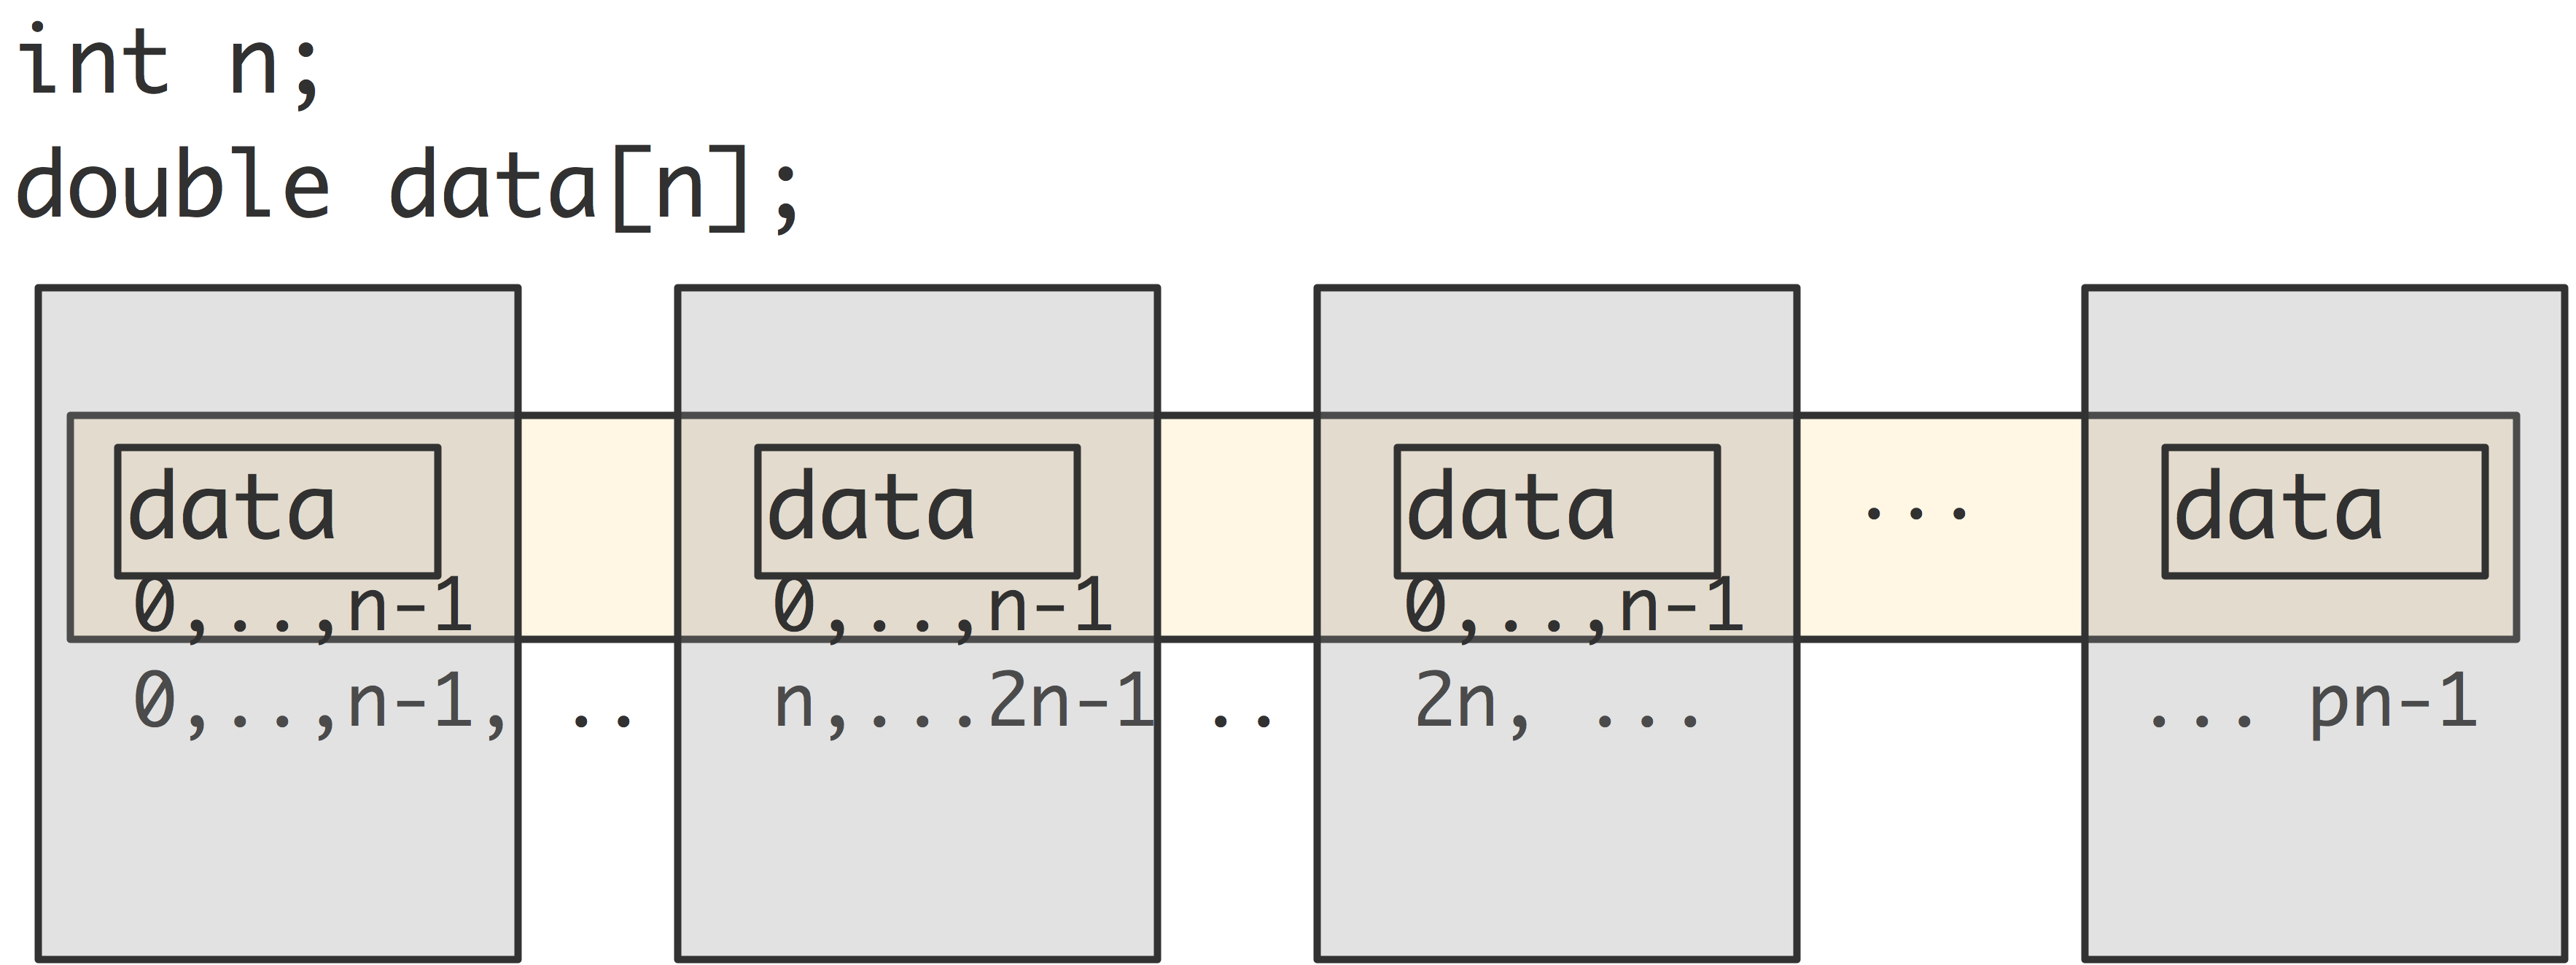
\includegraphics[scale=.1]{mpi-array}
  \caption{Local parts of a distributed array}
  \label{fig:mpi-array}
\end{figure}

We sometimes say that \n{data} is the local part
of a \indexterm{distributed array} with a total size of
$\mathtt{n}\cdot\mathtt{p}$
elements.
However, this array only exists
conceptually: each processor has an array with lowest index zero,
and you have to translate that yourself to an index in the global
array.
In other words, you have to write your code in such a way that
it acts like you're working with a large array that is distributed
over the processors, while
actually manipulating only the local arrays on the processors.

Your typical code then looks like

\begin{lstlisting}
int myfirst = .....;
for (int ilocal=0; ilocal<nlocal; ilocal++) {
   int iglobal = myfirst+ilocal;
   array[ilocal] = f(iglobal);
}
\end{lstlisting}

\begin{exercise}
  \label{ex:fft-vector}
  Implement a (very simple-minded) Fourier transform: if $f$ is a
  function on the interval $[0,1]$, then the $n$-th Fourier
  coefficient is
  \[ f_n\hat = \int_0^1 f(t)e^{-t/\pi}\,dt \]
  which we approximate by
  \[ f_n\hat = \sum_{i=0}^{N-1} f(ih)e^{-in/\pi} \]
  \begin{itemize}
  \item Make one distributed array for the $e^{-inh}$ coefficients,
  \item make one distributed array for the $f(ih)$ values
  \item calculate a couple of coefficients
  \end{itemize}
\end{exercise}

\begin{comment}
  \begin{exercise}
    \label{ex:sumsquares}
    We want to compute $\sum_{n=1}^Nn^2$, and we do that as follows
    by filling in an array and summing the elements. (Yes, you can do it
    without an array, but for purposes of the exercise do it with.)

    Set a variable \n{N} for the total length of the array, and compute
    the local number of elements. Make sure you handle the case where
    $N$ does not divide perfectly by the number of processes.

    \begin{itemize}
    \item Now allocate the local parts: each processor should allocate
      only local elements, not the whole vector.\\
      (Allocate your array as real numbers. Why are integers not a good idea?)
    \item On each processor, initialize the local array
      so that the $i$-th location of the distributed array
      (for $i=0,\ldots,N-1$)
      contains~$(i+\nobreak 1)^2$.
    \item Now use a collective operation to compute the sum of the array values.
      The right value is $(2N^3+3N^2+N)/6$. Is that what you get?
    \end{itemize}
    (Note that computer arithmetic is not exact: the computed sum will
    only be accurate up to some relative accuracy.)
  \end{exercise}
\end{comment}

\begin{exercise}
  In the previous exercise you worked with a distributed array,
  computing a local quantity and combining that into a global
  quantity.
  Why is it not a good idea to gather the whole distributed array on a
  single processor, and do all the computation locally?
\end{exercise}

If the array size is not perfectly divisible by the number of processors,
we have to come up with a division that is uneven, but not too much.
You could for instance, write

\begin{lstlisting}
int Nglobal, // is something large
    Nlocal = Nglobal/ntids,
    excess = Nglobal%ntids;
if (mytid==ntids-1) 
  Nlocal += excess;
\end{lstlisting}

\begin{exercise}
  Argue that this strategy is not optimal. Can you come up with a
  better distribution?
  Load balancing is further discussed in~\HPSCref{sec:load}.
\end{exercise}

\begin{comment}
  \begin{exercise}
    \label{ex:inproduct}
    Implement an inner product routine: let $x$ be a
    distributed vector of size~$N$ with elements $x[i]=i$,
    and compute~$x^tx$.
    As before, the right value is $(2N^3+3N^2+N)/6$.

    Use the inner product value to scale to vector so that it has
    norm~1.
    Check that your computation is correct.
  \end{exercise}
\end{comment}

%% \Level 0 {Blocking point-to-point operations}
\input chapters/mpi-blocksend

%% \Level 0 {Non-blocking point-to-point operations}
\input chapters/mpi-nonblock

\Level 0 {More about point-to-point communication}

\Level 1 {Message probing}
\label{sec:mpi-probe}

MPI receive calls specify a receive buffer, and its size has to be
enough for any data sent. In case you really have no idea how much data
is being sent, and you don't want to overallocate the receive buffer,
you can use a `probe' call.

The routine \indexmpiref{MPI_Probe} (and \indexmpishow{MPI_Iprobe},
for which see section~\ref{sec:progress}), accepts a message,
but does not copy the data. Instead, when probing tells you that there is a
message, you can use \indexmpishow{MPI_Get_count} to determine its size,
allocate a large enough receive buffer, and do a regular receive to
have the data copied.

\cverbatimsnippet[examples/mpi/c/probe.c]{probe}

There is a problem with the \indexmpishow{MPI_Probe} call in a
multithreaded environment: the following scenario can happen.
\begin{enumerate}
\item A thread determines by probing that a certain message has come
  in.
\item It issues a blocking receive call for that message\dots
\item But in between the probe and the receive call another thread
  has already received the message.
\item \dots~Leaving the first thread in a blocked state with not
  message to receive.
\end{enumerate}
This is solved by \indexmpiref{MPI_Mprobe}, which after a successful
probe removes the message from the \indexterm{matching queue}: the
list of messages that can be matched by a receive call. The thread
that matched the probe now issues an \indexmpiref{MPI_Mrecv} call on
that message through an object of type \indexmpidef{MPI_Message}.

\Level 1 {The Status object and wildcards}
\label{sec:mpi-wildcard}
\label{sec:mpi-status}
\index{message!status|(textbf}

In section~\ref{sec:mpi-send-recv}
you saw that \indexmpishow{MPI_Recv} has a `status' argument
of type \indexmpishow{MPI_Status} that \indexmpishow{MPI_Send} lacks.
(The various \indexmpishow{MPI_Wait...}  routines also have a status
argument; see section~\ref{sec:nonblocking}.)
Often you specify \indexmpishow{MPI_STATUS_IGNORE}
for this argument: commonly you know
what data is coming in and where it is coming from.

However, in some circumstances the recipient may not know all details of a
message when you make the receive call, so MPI has a way of querying
the \emph{status}\index{status!of received message} of the message:
\begin{itemize}
\item If you are expecting multiple incoming messages, it may be most
  efficient to deal with them in the order in which they arrive. So,
  instead of waiting for specific message, you would specify
  \indexmpishow{MPI_ANY_SOURCE} or \indexmpishow{MPI_ANY_TAG} in
  the description of the receive message. 
  Now you have to be able to ask `who did this message come from,
  and what is in it'.
\item Maybe you know the sender of a message, but the amount of data
  is unknown. In that case you can overallocate your receive buffer,
  and after the message is received ask how big it was, or you can
  `probe' an incoming message and allocate enough data when you find
  out how much data is being sent.
\end{itemize}

To do this, the receive call has a \indexmpidef{MPI_Status}
parameter.

This status is a property of the actually received messsage, so \indexmpishow{MPI_Irecv}
does not have a status parameter, but \indexmpishow{MPI_Wait} does.

\begin{mplnote}{Status object}
  The \lstinline+mpl::status+ object is created by the receive
  (or wait) call:

  \cxxverbatimsnippet{mplstatuscreate}

  A constant \lstinline+mpl::+\indexmplshow{any_source} exists.
\end{mplnote}

The \indexmpishow{MPI_Status} object
is a structure with freely accessible members,
as discussed below.

\Level 2 {Source}

In some applications it makes sense that a message can come from 
one of a number of processes. In this case, it is possible to specify
\indexmpishow{MPI_ANY_SOURCE} as the source.
%
To find out the \emph{source}\index{message!status!source}
where the message actually
came from, you would use the \indexmpishow{MPI_SOURCE} field of the status object
that is delivered by \indexmpishow{MPI_Recv} or the \indexmpishow{MPI_Wait...} call after an \indexmpishow{MPI_Irecv}.
\begin{lstlisting}
MPI_Recv(recv_buffer+p,1,MPI_INT, MPI_ANY_SOURCE,0,comm,
         &status);
sender = status.MPI_SOURCE;
\end{lstlisting}

The source of a message can be obttained as the
\indexmpidef{MPI_SOURCE}
member of the status structure.

There are various scenarios where receiving from `any source' makes sense.
One is that of the \indexterm{manager-worker} model. The manager task would first send
data to the worker tasks, then issues a blocking wait for the data of whichever process
finishes first.

This code snippet is a simple model for this: all workers processes wait
a random amount of time. For efficiency, the manager process accepts message from any source.

\cverbatimsnippet[examples/mpi/c/anysource.c]{anysource}

In Fortran2008 style, the source is a member of the \flstinline{Status} type.

\fverbatimsnippet[examples/mpi/f08/anysource.F90]{anysource-f08}

In Fortran90 style, the source is an index in the \flstinline{Status} array.

\fverbatimsnippet[examples/mpi/f/anysource.F90]{anysource-f}

\begin{mplnote}{Status querying}
The \indexmplshow{status} object can be queried:
\begin{lstlisting}
int source = recv_status.source();
\end{lstlisting}
\end{mplnote}

\Level 2 {Tag}

If a processor is expecting more than one messsage from a single other processor,
message tags are used to distinguish between them. In that case,
a value of \indexmpishow{MPI_ANY_TAG} can be used, and the actual
\emph{tag}\index{message!status!tag}
of a message can be retrieved as the
%
\indexmpidef{MPI_TAG}
%
member in the status structure. See the section about \clstinline+MPI_SOURCE+
for how to use this.

\begin{mplnote}{Message tag}
  \ac{MPL} differs from other \acp{API} in its treatment of tags:
  a~tag is not directly an integer, but an object of class \indexmplshow{tag}.
  %
  \cxxverbatimsnippet{mplsendrecv} % in an exercise
  %
  The \indexmplshow{tag} class has a couple of methods such as
  \lstinline+mpl::+\indexmplshow{tag::any}\lstinline+()+
  (for the \indexmpishow{MPI_ANY_TAG} wildcard in receive calls)
  and
  \lstinline+mpl::+\indexmplshow{tag::up}\lstinline+()+
  (for the \indexmpishow{MPI_TAG_UB} attribute).
\end{mplnote}

\Level 2 {Error}
\label{sec:mpi-status-error}

Any \emph{errors}\index{message!status!error}
during the receive operation can be found as the
\indexmpidef{MPI_ERROR}
member of the status structure.
This field is only set by functions that return multiple statuses,
such as \indexmpishow{MPI_Waitall}.
For functions that return a single status, any error is returned
as the function result.
For a function returning multiple statuses, the presence of any error
is indicated by a result of \indexmpishow{MPI_ERR_IN_STATUS}.

\Level 2 {Count}

If the amount of data received is not known a~priori, the
\emph{count}\index{message!count} of elements received
can be found by 
\indexmpiref{MPI_Get_count}:

This may be necessary since the \n{count} argument to \indexmpishow{MPI_Recv} is 
the buffer size, not an indication of the actually received number of
data items.

Remarks.
\begin{itemize}
\item Unlike the above, this is not directly a member of the status
  structure.
\item The `count' returned is the number of elements of the specified
  datatype. If this is a derived type
  (section~\ref{sec:derived-types}) this is not the same as the number
  of elementary datatype elements. For that, use
  \indexmpiref{MPI_Get_elements} or
  \indexmpishow{MPI_Get_elements_x}
  which returns the number of basic elements.
\end{itemize}

\begin{mplnote}{Receive count}
  The \lstinline+get_count+ function is a method of the status object.
  The argument type is handled through templating:
  %
  \cxxverbatimsnippet[examples/mpi/mpl/recvstatus.cxx]{mplrecvcount}
\end{mplnote}

\Level 2 {Example: receiving from any source}

Using the \indexmpishow{MPI_ANY_SOURCE} specifier. We retrieve the
actual source from the \indexmpishow{MPI_Status} object through the
\indexmpishow{MPI_SOURCE} field.
%
\cverbatimsnippet[examples/mpi/c/anysource.c]{anysource}
%
\pverbatimsnippet[examples/mpi/p/anysource.py]{anysourcep}

In sections \ref{prj:mandelbrot} and~\ref{sec:mpi-test} we explained
the \indexterm{manager-worker} model, and how it offers an opportunity for inspecting the
\indexmpishow{MPI_SOURCE} field of the \indexmpishow{MPI_Status}
object describing the data that was received.

\index{message!status|)}

\Level 0 {Review questions}

For all true/false questions, if you answer that a statement is false,
give a one-line explanation.

\begin{enumerate}
\item Describe a deadlock scenario involving three processors.

\item True or false: a message sent with \lstinline{MPI_Isend} from one processor can be
  received with an \lstinline{MPI_Recv} call on another processor.

\item True or false: a message sent with \lstinline{MPI_Send} from one processor can be
  received with an \lstinline{MPI_Irecv} on another processor.

\item Why does the \lstinline{MPI_Irecv} call not have an \lstinline{MPI_Status} argument?

\item
  Suppose you are testing ping-pong timings.
  Why is it generally not a good idea to use processes 0 and~1 for the
  source and target processor?  Can you come up with a better guess?

%% one-sided
\item What is the relation between the concepts of `origin', `target', `fence',
  and `window' in one-sided communication.

\item What are the three routines for one-sided data transfer?

\lstset{
  style=reviewcode,
  language=C,
}

\item In the following fragments % in figures~\ref{fig:qblockc},\ref{fig:qblockf},
  assume that all buffers have been
  allocated with sufficient size. For each fragment note whether it
  deadlocks or not. Discuss performance issues.

    \lstset{language=C,basicstyle=\footnotesize\ttfamily}
    %% \lstinputlisting{qblock1}
\begin{lstlisting}
for (int p=0; p<nprocs; p++)
  if (p!=procid)
    MPI_Send(sbuffer,buflen,MPI_INT,p,0,comm);
for (int p=0; p<nprocs; p++)
  if (p!=procid)
  MPI_Recv(rbuffer,buflen,MPI_INT,p,0,comm,MPI_STATUS_IGNORE);
\end{lstlisting}
    %% \lstinputlisting{qblock2}
\begin{lstlisting}
for (int p=0; p<nprocs; p++)
  if (p!=procid)
    MPI_Recv(rbuffer,buflen,MPI_INT,p,0,comm,MPI_STATUS_IGNORE);
for (int p=0; p<nprocs; p++)
  if (p!=procid)
  MPI_Send(sbuffer,buflen,MPI_INT,p,0,comm);
\end{lstlisting}
    %% \lstinputlisting{qblock3}
\begin{lstlisting}
int ireq = 0;
for (int p=0; p<nprocs; p++)
  if (p!=procid)
    MPI_Isend(sbuffers[p],buflen,MPI_INT,p,0,comm,&(requests[ireq++]));
for (int p=0; p<nprocs; p++)
  if (p!=procid)
    MPI_Recv(rbuffer,buflen,MPI_INT,p,0,comm,MPI_STATUS_IGNORE);
MPI_Waitall(nprocs-1,requests,MPI_STATUSES_IGNORE);
\end{lstlisting}
    %% \lstinputlisting{qblock4}
\begin{lstlisting}
int ireq = 0;
for (int p=0; p<nprocs; p++)
  if (p!=procid)
    MPI_Irecv(rbuffers[p],buflen,MPI_INT,p,0,comm,&(requests[ireq++]));
for (int p=0; p<nprocs; p++)
  if (p!=procid)
    MPI_Send(sbuffer,buflen,MPI_INT,p,0,comm);
MPI_Waitall(nprocs-1,requests,MPI_STATUSES_IGNORE);
\end{lstlisting}
    %% \lstinputlisting{qblock5}
\begin{lstlisting}
int ireq = 0;
for (int p=0; p<nprocs; p++)
  if (p!=procid)
    MPI_Irecv(rbuffers[p],buflen,MPI_INT,p,0,comm,&(requests[ireq++]));
MPI_Waitall(nprocs-1,requests,MPI_STATUSES_IGNORE);
for (int p=0; p<nprocs; p++)
  if (p!=procid)
    MPI_Send(sbuffer,buflen,MPI_INT,p,0,comm);
\end{lstlisting}

    \pagebreak
    Fortran codes:
    
    \lstset{style=reviewcode,language=Fortran}

  \lstset{language=Fortran,basicstyle=\footnotesize\ttfamily}
  %% \lstinputlisting{qblock1f}
\begin{lstlisting}
do p=0,nprocs-1
   if (p/=procid) then
      call MPI_Send(sbuffer,buflen,MPI_INT,p,0,comm,ierr)
   end if
end do
do p=0,nprocs-1
   if (p/=procid) then
      call MPI_Recv(rbuffer,buflen,MPI_INT,p,0,comm,MPI_STATUS_IGNORE,ierr)
   end if
end do
\end{lstlisting}
  %% \lstinputlisting{qblock2f}
\begin{lstlisting}
do p=0,nprocs-1
   if (p/=procid) then
      call MPI_Recv(rbuffer,buflen,MPI_INT,p,0,comm,MPI_STATUS_IGNORE,ierr)
   end if
end do
do p=0,nprocs-1
   if (p/=procid) then
      call MPI_Send(sbuffer,buflen,MPI_INT,p,0,comm,ierr)
   end if
end do
\end{lstlisting}
  %% \lstinputlisting{qblock3f}
\begin{lstlisting}
ireq = 0
do p=0,nprocs-1
   if (p/=procid) then
      call MPI_Isend(sbuffers(1,p+1),buflen,MPI_INT,p,0,comm,&
           requests(ireq+1),ierr)
      ireq = ireq+1
   end if
end do
do p=0,nprocs-1
   if (p/=procid) then
      call MPI_Recv(rbuffer,buflen,MPI_INT,p,0,comm,MPI_STATUS_IGNORE,ierr)
   end if
end do
call MPI_Waitall(nprocs-1,requests,MPI_STATUSES_IGNORE,ierr)
\end{lstlisting}
  %% \lstinputlisting{qblock4f}
\begin{lstlisting}
ireq = 0
do p=0,nprocs-1
   if (p/=procid) then
      call MPI_Irecv(rbuffers(1,p+1),buflen,MPI_INT,p,0,comm,&
           requests(ireq+1),ierr)
      ireq = ireq+1
   end if
end do
do p=0,nprocs-1
   if (p/=procid) then
      call MPI_Send(sbuffer,buflen,MPI_INT,p,0,comm,ierr)
   end if
end do
call MPI_Waitall(nprocs-1,requests,MPI_STATUSES_IGNORE,ierr)
\end{lstlisting}
  %% \lstinputlisting{qblock5f}
\begin{lstlisting}
// block5.F90
ireq = 0
do p=0,nprocs-1
   if (p/=procid) then
      call MPI_Irecv(rbuffers(1,p+1),buflen,MPI_INT,p,0,comm,&
           requests(ireq+1),ierr)
      ireq = ireq+1
   end if
end do
call MPI_Waitall(nprocs-1,requests,MPI_STATUSES_IGNORE,ierr)
do p=0,nprocs-1
   if (p/=procid) then
      call MPI_Send(sbuffer,buflen,MPI_INT,p,0,comm,ierr)
   end if
end do
\end{lstlisting}

\item Consider a ring-wise communication where
\begin{lstlisting}
int
  next = (mytid+1) % ntids,
  prev = (mytid+ntids-1) % ntids;
\end{lstlisting}
  and each process sends to \lstinline{next}, and receives from \lstinline{prev}.

  The normal solution for preventing deadlock is to use both
  \indexmpishow{MPI_Isend} and \indexmpishow{MPI_Irecv}. The send and
  receive complete at the wait call. But does it matter in what
  sequence you do the wait calls?
  \begin{multicols}{2}
    \cverbatimsnippet{ring3}
    \columnbreak
    \cverbatimsnippet{ring4}
  \end{multicols}

  Can we have one non-blocking and one blocking call?
  Do these scenarios block?
  \begin{multicols}{2}
    \cverbatimsnippet{ring1}
    \columnbreak
    \cverbatimsnippet{ring2}
  \end{multicols}
\end{enumerate}

\index{communication!two-sided|)}
